\chapter{DCC File Format Description} \label{app:dccspec}

\begin{centering}
\large{by Bilian Belchev and Paul Siramy}\\
\end{centering}

\vspace{1cm}
NOTE: \href{http://paul.siramy.free.fr/_divers/dcc_doc.zip}{This document has been copied from paul.siramy.free.fr}


\paragraph{READ THIS FIRST}
According to the END USER LICENSE of Diablo II and Diablo II Lord of Destruction 
it's illegal to "copy, photocopy, reproduce, translate, reverse engineer, derive 
source code, modify, disassemble, decompile, create derivative works based on 
the Program". Mod making includes copying (patches and modified archives are 
parts of the Program), reverse engineering, modifying and even more. So 
mod-making is illegal.

But in an interview Bill Roper of Blizzard Entertainment 
said that they were "always intrigued and interested in the mods people make" 
and they had no problems with total conversions of their games, so long as they 
are for personal use. So it turns out that mod making is not so illegal. I am a 
devoted player of Diablo and Diablo II and also a programmer. I program on my 
own; I am not a professional programmer yet (although I desire to be). 

This document is intended to help mod-makers and programmers that make tools for 
mod-making or just help the fans of Diablo II view the graphic files of the 
game. So I don't look upon my work as something illegal. I have no desire to do 
any harm to the great game or to its authors. 

\textbf{
THIS DOCUMENT MUST BE USED FOR PERSONAL AND NON COMMERCIAL PURPOSES ONLY! THIS 
DOCUMENT IS PROVIDED "AS IS" WITHOUT WARRANTY OF ANY KIND. I DO NOT TAKE ANY 
RESPONSIBILYTY IF THIS DOCUMENT IS IMPROPERLY USED.
}

\todo{The original DCC doc could use re-wording for clarity}

\newpage
\section{Overview}
The Dcc files are used in Diablo II for storing images - frames and animations.
This document contains a description of how the Dcc files are structured, how 
to decompress images from them and even some tips for creating Dcc files.

\subsection{File Structure}
\begin{figure}[h!]
	\caption{Description of the byte offsets of variables inside of a DCC file.}

	\vspace{0.25cm}

	\begin{tabular}{|c|c|c|}
	Offset in File & Variable Name & Variable Type \\
	\hline
	0x00 & Signature & Byte \\
	0x01 & Version & Byte \\
	0x02 & NumDirections & Byte \\
	0x03 & NumFrames & DWORD \\
	0x07 & One & DWORD \\
	0x0b & TotalSizeCoded & DWORD \\
	0x0f & DirOffset[0] & DWORD \\
	\ldots & \ldots & \ldots \\
	0x0f + (NumDirections-1)*4 & DirOffset[NumDirections-1] & DWORD \\
	DirOffset[0] & Direction[0] Data & Bitstream \\
	\ldots & \ldots & \ldots \\
	DirOffset[NumDirections-1] & Direction[NumDirections-1] Data & Bitstream \\
	\end{tabular}

\end{figure}


\paragraph{Signature} -- A value of 0x74 means this is a Dcc file. If the value 
is not 0x74 Diablo II doesn't render any frames from this file on the screen - 
it just ignores the file.	

\paragraph{Version} -- It seems that it is always equal to 0x06. However other 
values behave the same way as 0x06. Maybe future versions of the format will 
actually use this variable.	

\paragraph{NumDirections} -- The number of directions in the file. The following 
values are used: 1 (0x01), 4 (0x04), 8 (0x08), 16 (0x10) and 32 (0x20). A value 
larger then 32 will cause an Assertion Failure!	

\paragraph{NumFrames} -- The number of frames in each direction in the file. The 
minimum value is 0 (it shouldn't crash the game) and the maximum is 256.	

\paragraph{One} -- Paul Siramy has checked that this variable is always 1 in 
all the Dcc files from Diablo II that are originally created by Blizzard 
Entertainment. However the purpose of this variable is still unknown.	

\paragraph{TotalSizeCoded} -- This variable seems to be always equal to the sum 
of all the OutSizeCoded variables (from all directions) + NumDirections*NumFrames*4 
+ 24.	

\paragraph{DirOffset[0]} -- A file offset of the first direction (direction0) 
data. It is followed by the file offset of the second direction data (only if 
NumDirections>1) and so on. Immediately after the last offset the data of the 
first direction begin. (In fact you can use a larger offset so you can insert 
additional bytes here but they will never be used so what's the sense?)	

\paragraph{Direction[0] Data} -- The data for the first direction. You can 
calculate the size in bytes subtracting the file offset of this direction from 
the file offset of the next direction. The next section describes how the data 
is actually structured.

\subsection{Bitstream Structure}

\vspace{0.25cm}
\hspace{-1cm} % this is a wide fucking table
\begin{tabular}{|c|c|c|}\fontsize{4}{5}
Variable Name & Variable Type & Variable Size (in bits) \\
\hline
OutSizeCoded & DWORD & 32 \\
CompressionFlags & 2 bits & 2 \\
Variable0Bits & Unisgned Integer & 4 \\
WidthBits & Unisgned Integer & 4 \\
HeightBits & Unisgned Integer & 4 \\
XOffsetBits & Unisgned Integer & 4 \\
YOffsetBits & Unisgned Integer & 4 \\
OptionalDataBits & Unisgned Integer & 4 \\
CodedBytesBits & Unisgned Integer & 4 \\
Variable0 & Unisgned Integer & Variable0Bits \\
Width & Unisgned Integer & WidthBits \\
Height & Unisgned Integer & HeightBits \\
XOffset & Signed Integer & XOffsetBits \\
YOffset & Signed Integer & YOffsetBits \\
NumOptionalBytes & Unsigned Integer & OptionalDataBits \\
NumCodedBytes & Unsigned Integer & CodedBytesBits \\
FrameBottomUp & Flag & 1 \\
Next Frames & \ldots & \ldots \\
Align & value not used & (see below) \\
Frame[0] Optional Data & Bytes & 8*(Frame[0]NumOptionalBytes) \\
\ldots & \ldots & \ldots \\
Frame[NumFrames-1] Optional Data & Bytes & 8*(Frame[NumFrames-1]NumOptionalBytes) \\
EqualCellsBitstreamSize & Unsigned Integer & 20 \\
PixelMaskBitstreamSize & Unsigned Integer & 20 \\
EncodingTypeBitstreamSize & Unsigned Integer & 20 \\
RawPixelCodesBitstreamSize & Unsigned Integer & 20 \\
PixelValuesKey & 256 bits & 256 \\
EqualCellsBitstream  &  Bitstream  &  EqualCellsBitstreamSize  \\
PixelMaskBitstream  &  Bitstream  &  PixelMaskBitstreamSize  \\
EncodingTypeBitstream  &  Bitstream  &  EncodingTypeBitstreamSize  \\
RawPixelCodesBitstream  &  Bitstream  &  RawPixelCodesBitstreamSize  \\
PixelCodesAndDisplacementBitstream & Bitstream & Unknown (to end of data) \\
\end{tabular}


\paragraph{OutSizeCoded} -- A DWORD value that indicates how much memory the 
decompressor must allocate to hold the output data for this direction. The 
output data consist of decompressed frame information (frame header) for each 
frame of the NumFrames and the encoded frame data for each frame. That's right 
the decompressor encodes the decompressed pixels before they are used. The 
encoding scheme is quite simple: if we have N pixels that are transparent 
(color index 0) we write the value 0x80|N (the maximum value of N is 127 and 
the minimum is 1 (the code 0x80 means end of current scanline)), else if we 
have M non transparent pixels we write the code M (the maximum value of M is 
127 and the minimum is 1 (byte 0x00 is not used)) followed by the pixel values 
of the M pixels. If all the pixels in the rest of the scanline are transparent 
we write the code 0x80 (end of current scanline) and continue with the next 
scanline. If there are more than 127 consecutive transparent or non-transparent 
pixels we encode 127 of them and then the rest of them (we can repeat this 
several times). However you only need to calculate this variable when you 
create Dcc files. Use the following formula: 32 (size of the frame header)+size 
of encoded scanlines of this frame +3 (padding bytes) and repeat this for all 
the NumFrames (+32 +size of...+3 +32 +size of... +3 +...).	

\paragraph{CompressionFlags} -- If bit1 is set the variables 
EqualCellsBitstreamSize and EqualCellsBitstream are present in this bitstream, 
else they must be skipped (because they are not present) when the stream is 
analyzed. If bit0 is set the variables EncodingTypeBitsreamSize, 
RawPixelCodesBitstreamSize, EncodingTypeBitsream and RawPixelCodesBitstream are 
present in this bitstream, else they must be skipped.	

\paragraph{Variable0Bits} -- This is a 4-bit code that indicates how many 
significant bits each Variable0 (from each frame header) contains. These 4 bits 
contain only a code, so the following table must be used to obtain the actual 
number of significant bits in each Variable0.

\vspace{0.25cm}
\begin{tabular}{|c|c|}
Value of the 4-bit code & Actual number of significant bits \\
\hline
0x0 & 0 \\
0x1 & 1 \\
0x2 & 2 \\
0x3 & 4 \\
0x4 & 6 \\
0x5 & 8 \\
0x6 & 10 \\
0x7 & 12 \\
0x8 & 14 \\
0x9 & 16 \\
0xa & 20 \\
0xb & 24 \\
0xc & 26 \\
0xd & 28 \\
0xe & 30 \\
0xf & 32 \\
\end{tabular}




\paragraph{WidthBits} -- A 4-bit code that indicates how many significant bits 
each Width variable (from each frame header) contains. The same table as above 
must be used.	

\paragraph{HeightBits} -- Again a 4-bit code - indicates how many significant 
bits each Height variable (from each frame header) contains. (See Variable0Bits 
for details.)	

\paragraph{XOffsetBits} -- Again a 4-bit code - indicates how many significant 
bits each XOffset variable (from each frame header) contains. (See Variable0Bits 
for details.)	

\paragraph{YOffsetBits} -- Again a 4-bit code - indicates how many significant 
bits each YOffset variable (from each frame header) contains. (See Variable0Bits 
for details.)	

\paragraph{OptionalDataBits} -- Again a 4-bit code - indicates how many 
significant bits each NumOptionalBytes variable (from each frame header) 
contains. (See Variable0Bits for details.)	

\paragraph{CodedBytesBits} -- Again a 4-bit code - indicates how many 
significant bits each NumCodedBytes variable (from each frame header) contains. 
(See Variable0Bits for details.)	

\paragraph{Variable0} -- The first variable of the frame header. Its value is 
not used by the decompressor but the value is always written in the output data. 
If you just decode Dcc files there is no need to evaluate this variable. If you 
create your own Dcc files set this variable to 0.	
All variables colored in orange form a frame header. Each direction's data 
contain a frame header for each frame in that direction (because all directions 
contain the same number of frames the data of each direction contain NumFrames 
frame headers). The first frame header is the frame header of frame 0. It's 
followed by the frame header of frame 1 and so on.	

\paragraph{Width} -- The width in pixels of the frame.	

\paragraph{Height} -- The height in pixels of the frame.	

\paragraph{XOffset} -- All frames are rendered on the screen relative to one 
base point. This is a signed variable that indicates how many pixels right (left 
if the value is negative) of the base point the frame will be rendered on the 
screen. Warning! This is a signed value. The most significant of the loaded bits 
contains the sign. After you have loaded and zero extended this variable to fit 
your 16 or 32 bit variable you have to analyze the most significant of the 
loaded bits - if it is set you have to set all bits that are not loaded to 1 
(they are set to 0) else (the most significant of the loaded bits is not set) 
the variable doesn't need to be corrected.	

\paragraph{YOffset} -- A signed variable that indicates how many pixels down 
(up if the value is negative) of the base point the frame will be rendered on 
the screen. However it is not that simple - this value depends on FrameBottomUp 
(see the Frames and Offsets section below). Warning! This is a signed value. 
See XOffset for details how to convert it to 16 or 32 bit variable.	

\paragraph{NumOptionalBytes} -- Indicates how many bytes must be loaded and 
written in the output data as additional bytes of data for this frame (frame 
optional data). This variable usually has a value of 0 (means this frame has no 
additional data).	

\paragraph{NumCodedBytes} -- The amount of bytes required to hold the coded 
scanlines for this frame. The encoding scheme is described already in this 
document. (See OutSizeCoded above.)	

\paragraph{FrameBottomUp} -- If this bit is set to 1 the frame is encoded as 
bottom-up frame - the origin of the frame is its lower-left corner and the frame 
has to be flipped along its x-axis in order to be used. If this bit is 0 the 
frame is encoded as top-down frame - the origin of the frame is in its 
upper-left corner and no flipping is required. Warning! This flag is used during 
decompression so you can't just change it in order to just flip the image this 
frame contains.	

\paragraph{align} -- If there is a frame that contains additional data 
(NumOptionalBytes for that frame is not 0) this field is used in order to align 
the optional data on a byte boundary. If there is no frame that contains 
additional data this field is not present in the bitstream (there is no need 
EqualCellsBitstreamSize to be aligned on any boundary).	

\paragraph{Frame 0 Optional Data} -- If there are frames that contain additional 
data after the align field the additional data for the first frame that contains 
such data is stored. It is followed by the additional data of the next frame 
that contains additional data (only if there is such a frame) and so on.	

\paragraph{EqualCellsBitstreamSize} -- A 20-bit value that indicates how long 
the EqualCellsBitstream is (in bits). This variable is only present if bit1 of 
CompressionFlags is set to 1.	

\paragraph{PixelMaskBitstreamSize} -- A 20-bit value that indicates how long the 
PixelMaskBitstream is (in bits).	

\paragraph{EncodingTypeBitsreamSize} -- A 20-bit value that indicates how long 
the EncodingTypeBitsream is (in bits). This variable is only present if bit0 of 
CompressionFlags is set to 1.	

\paragraph{RawPixelCodesBitstreamSize} -- A 20-bit value that indicates how long 
the RawPixelCodesBitstream is (in bits). This variable is only present if bit0 
of CompressionFlags is set to 1.	

\paragraph{PixelValuesKey} -- 256 bits that indicate which of the 256 colors in 
the palette are used. For example if color 57 is used in the frames bit57 is set 
to 1 else if color 57 is not used bit57 is set to 0. If there are any 
transparent pixels in the frames bit0 must be set to 1 (color index 0 is used 
for transparency). This 256 key is used to translate the stored pixel codes to 
valid pixel values. Example: imagine a Dcc file that contains only a few small 
frames and the used colors are: 0 (transparency), 27,41,56 and 85. So the 
decompressor reads the key and when it decodes a pixel code of 0 it transforms 
it to pixel value of 0, when it decodes a pixel code 1 it transforms it to pixel 
value 27, when it decodes a pixel code 2 it transforms it to pixel value 41 and 
so on (3 to 56 and 4 to 85).	

\paragraph{EqualCellsBitstream} -- If the decompressor reached a cell (cell - 
a piece of frame - its dimensions vary from 1 to 5 (usually 4x4 but also 1x1, 
1x3, 2x3, 5x2, etc.) according to where the cell is in the frame) 
that was previously decoded it analyzes (loads) one bit from this bitstream to 
determine if the reached cell is the same as the previously decoded one, or if 
the cells have different dimensions if the new cell is completely transparent. 
If the loaded bit has a value of 1 the new cell is the same as the previously 
decoded one or the new cell is completely transparent.

\newpage
\section{Frames and Offsets}
Since there is no dependency between the direction data bitstreams of different 
directions in one and the same Dcc file, that bitstreams can be processed 
independently. In fact that is actually the case. The game decompresses the 
data for a particular direction from a particular Dcc file only if it needs the 
frames that direction contains. For example if the player enters the game, 
shoots only once in a particular direction and exits the game probably the game 
will decompress the frames for the arrow only for that direction. So below 
except if other is noted, we will look at the frames for a particular direction 
only.

In general all the frames of one direction are of different sizes and have 
different offsets. The X offset (from the frame header in the Dcc file) always 
specifies how many pixels right of the base point, the left edge of the frame 
is. If the frame is a top-down frame (the FrameBottomUp flag in the frame header 
is not set) the Y offset (the one from the frame header) specifies how many 
pixels down from the base point, the bottom edge (or the bottom-left corner, if 
you prefer) of the frame is. Here is an example:

\graphicspath{{./image/dcc/}}
\begin{figure}[!h]
  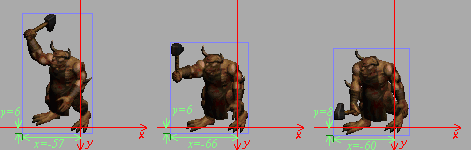
\includegraphics[width=\linewidth]{top.png}
  \caption{
The red axes are the axes for rendering on the screen. The point that 
they intersect is the base point on the screen. However these taken directly 
from the frame headers per frame offsets are not the ones used for rendering on 
the screen. They must not be misidentified with the offsets for the different 
directions that have to be passed to the cvdcc add-on for Cv5 when saving Dcc 
files. These offsets are used for frame alignment during the decompression and 
also to calculate the offsets for rendering on the screen.}
  \label{fig:top}
\end{figure}

\begin{figure}[!h]
  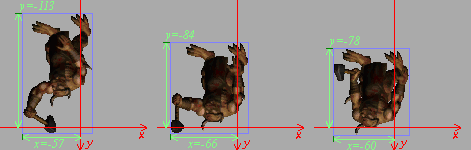
\includegraphics[width=\linewidth]{bottom.png}
  \caption{
However if the FrameBottomUp flag from the frame header is set that frame is 
encoded as bottom-up frame. In this case the Y offset tells the decompressor 
how many pixels down from the base point, the bottom edge of the image is. Since 
in this case the frame is flipped vertically the Y offset specifies the 
displacement of the top edge of the frame. See this example:
}
  \label{fig:bottom}
\end{figure}

	
\begin{figure}[!h]
  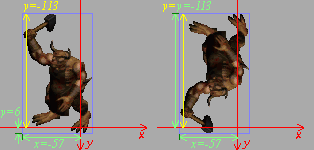
\includegraphics[width=\linewidth]{scroffs.png}
  \caption{
Note that since the output of the decompressor is the same for the both cases 
(it is like the second image) the screen offsets are also the same. The offsets 
you have to pass to the cvdcc add-on are the screen offsets but for the frames 
you see in the viewer and the animator. They are for the whole frames not for 
the smallest rectangles that contain all the non-transparent pixels.
}
  \label{fig:offsets}
\end{figure}


\newpage
\section{The Frame Buffer}
Imagine the game renders all the frames for a particular direction (of a 
particular animation) at the appropriate positions (aligned according to the 
offsets from the base point), but one above another in one and the same of the 
large full screen frames (normally this never occurs, but imagine it for the 
purpose of our explanation). In that case it is very probable, that each next 
frame the game renders above the previous ones, overwrites portions of the 
previously rendered frames. Note that in some animations, if not the most then 
a significant part of the overwritten pixels will be the same as those that 
overwrite them. Making such considerations it is not difficult to conclude that 
even whole parts of the frames (several adjacent pixels) will be the same 
between some consecutive frames. The Dcc format takes advantage of this fact. 
That is so the algorithm for Dcc decompression we are going to discuss uses a 
frame buffer, in which it constructs the frames consecutively.

Since in general all the frames are of different dimensions and positions, the 
dimensions of the frame buffer have to be determined in a such way that it can 
hold all the frames when rendered appropriately relative to each other (as on 
screen). Given the dimensions and the positions of all the frames it is not 
difficult to determine the offsets (according to the base point) of each of the 
edges of the smallest rectangle that bounds all the frames. Look at this 
picture:

\begin{figure}[!h]
  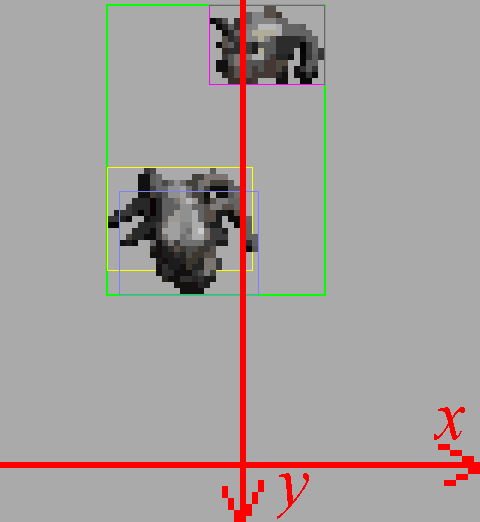
\includegraphics[width=\linewidth]{frmbuff.png}
  \caption{
The green rectangle shows the borders of the frame buffer. The frames are 
intentionally enlarged for better viewing. However these are only three of the 
frames. I have intentionally selected them - they are the most outlying ones so 
they have common edges with the frame buffer. In this example the width of the 
frame buffer is 36 and the height is 48.
}
  \label{fig:framebuffer}
\end{figure}


\newpage
\section{The Cells}
The green lines show the default boundaries of the cells. There is no 
requirement the frame buffer to have width and height that are multiples of four 
as there is no requirement for the frames to be aligned on cell boundaries. If 
the width of the frame buffer is not a multiple of four then the last cells of 
each row of cells (we assume left to right ordering of the cells, and top to 
town in vertical) will have different dimensions. Analogically if the height is 
not a multiple of four the cells at the bottom of the frame buffer will have 
dimensions different than 4x4. However this is only the way the frame buffer is 
divided. There are additional conditions that specify the cell sizes for each 
frame.

\begin{figure}[!h]
  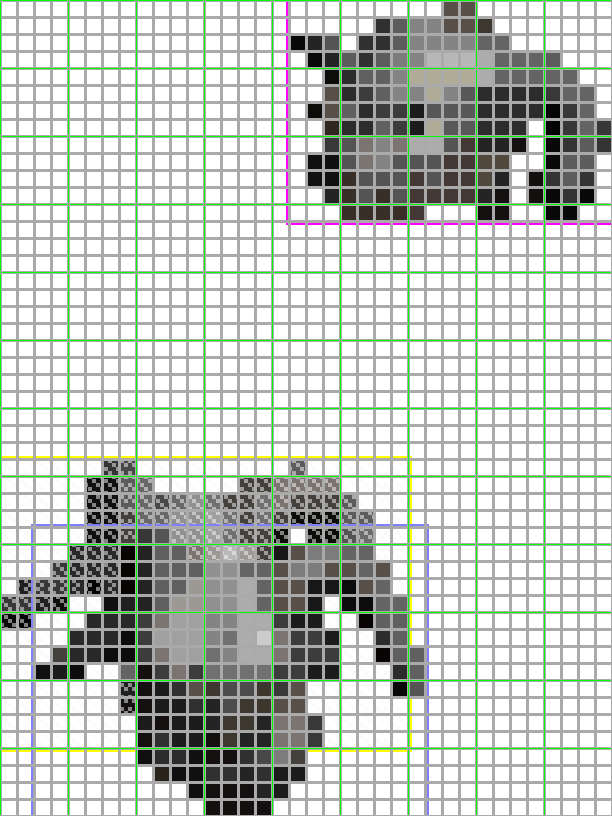
\includegraphics[width=\linewidth]{cels.png}
  \caption{
The frame buffer is divided into parts called cells. In general the entire frame 
buffer is divided into cells with dimensions of 4x4 as shown in this picture.
}
  \label{fig:cells}
\end{figure}

If there are no pixels from the cell, which results from the default division of 
the frame buffer, that are outside of the frame the cell has the default size of 
4x4. If there are pixels from that cell that are outside of the frame the 
corresponding cell from that frame has such dimensions that it contains pixels 
that are within the frame only. However there is one exception: if the last 
column or row of cells, produced by the default frame buffer division that have 
common pixels with the frame, have width of one or height of one respectively - 
the cells that are next to them and within the frame at the same time have width 
of 5 or height of 5 respectively. In fewer words this means the last cell in the 
row of the frame can't have width of one - in that case the cell left of it has 
width of 5. Analogically the cells at the bottom of the frame can't have height 
of one - instead the cells up of them have height of 5. However the width of a 
cell can't be greater than the width of the frame. The same applies for the 
height of a cell - must be smaller or equal to the height of the frame. So if we 
have a frame that have dimensions of 2x3 and it is placed in the frame buffer 
such that its pixel at the bottom-right corner of the frame is a pixel in the 
top-left corner of a cell - that frame will have only one cell with dimensions 
of 2x3 instead of four cells with dimensions of 1x2, 1x2, 1x1, 1x1.

Let's take look at the first frame (the one with the magenta border) 
in the frame buffer in \textbf{Figure \ref{fig:cells}}. 
Its first cell will have dimensions of 3x4 because the first column of the cell, 
produced by the default division, is outside of the frame. The next four cells 
of that frame will have the default dimensions - 4x4. The second row of cells 
for that frame is the same as the first (I mean the dimensions only). However 
the third row of cells will have height of 5, because if it has height of 4 only 
one row of pixels remain and the cells in the bottom of the frame will have 
height of 1. So for the frame with pink border we have:

\begin{table}[!h]
	\centering
	\begin{tabular}{|p{0.6cm}|p{1cm}|p{1cm}|p{1cm}|p{1cm}|}
		\hline
		& & & & \\[0.5cm] % a fake row with no hline, "extends" the cell
		3x4 & 4x4 & 4x4 & 4x4 & 4x4 \\
		\hline
		& & & & \\[0.5cm]
		3x4 & 4x4 & 4x4 & 4x4 & 4x4 \\
		\hline
		& & & & \\[1cm]
		3x5 & 4x5 & 4x5 & 4x5 & 4x5 \\
		\hline
	\end{tabular}
	\label{fig:cellstable1}
	\caption{ 
		The cells from the magenta frame in \textbf{Figure \ref{fig:cells}}.  
	}
\end{table}

	
Although the firs row of pixels in the frame with the yellow border lie in a 
separate row of cells (according to the default division of the frame buffer), 
there will be no first row of cells with height of 5 because this isn't at the 
left or bottom edge of the frame and the exception applies only to those edges. 
So for the frame with yellow border we have:

\begin{table}[!h]
	\centering
	\begin{tabular}{|p{0.6cm}|p{1cm}|p{1cm}|p{1cm}|p{1cm}|p{1.2cm}|}
		\hline
		2x1 & 4x1 & 4x1 & 4x1 & 4x1 & 4x1 \\
		\hline
		& & & & & \\[0.5cm]
		2x4 & 4x4 & 4x4 & 4x4 & 4x4 & 4x4 \\
		\hline
		& & & & & \\[0.5cm]
		2x4 & 4x4 & 4x4 & 4x4 & 4x4 & 4x4 \\
		\hline
		& & & & & \\[0.5cm]
		2x4 & 4x4 & 4x4 & 4x4 & 4x4 & 4x4 \\
		\hline
		& & & & & \\[0.5cm]
		2x4 & 4x4 & 4x4 & 4x4 & 4x4 & 4x4 \\
		\hline
	\end{tabular}
	\label{fig:cellstable2}
	\caption{ 
		The cells from the yellow frame in \textbf{Figure \ref{fig:cells}}.  
	}
\end{table}


	
And for the frame with blue border we have Table \ref{fig:cellstables3}.

\begin{table}[!h]
	\centering
	\begin{tabular}{|p{0.4cm}|p{1cm}|p{1cm}|p{1cm}|p{1cm}|p{1cm}|}
		\hline
		2x1 & 4x1 & 4x1 & 4x1 & 4x1 & 4x1 \\
		\hline
		& & & & & \\[0.5cm]
		2x4 & 4x4 & 4x4 & 4x4 & 4x4 & 4x4 \\
		\hline
		& & & & & \\[0.5cm]
		2x4 & 4x4 & 4x4 & 4x4 & 4x4 & 4x4 \\
		\hline
		& & & & & \\[0.5cm]
		2x4 & 4x4 & 4x4 & 4x4 & 4x4 & 4x4 \\
		\hline
		& & & & & \\[0.5cm]
		2x4 & 4x4 & 4x4 & 4x4 & 4x4 & 4x4 \\
		\hline
	\end{tabular}
	\label{fig:cellstable3}
	\caption{ 
		The cells from the blue frame in \textbf{Figure \ref{fig:cells}}.  
	}
\end{table}


	
Each cell from a particular frame corresponds to unique cell from the frame 
buffer - that unique cell is the cell that contains all the pixels from the cell 
from that particular frame or if there is no such cell (that is in the case 
where at least one of the dimensions of the cell from the frame is 5) - the cell 
from that particular frame is considered to correspond to the cell from the 
frame buffer that contains the most of the pixels. When two cells from different 
frames correspond to one and the same cell from the frame buffer these two cells 
are considered one and the same cell without regard of their dimensions (their 
dimensions can be different). In this way the first cell from the frame with the 
blue border (2x1) is considered to be the same cell as the first cell from the 
second row of cells from the frame with the yellow border (4x4).

\newpage
\section{The Actual Decompression}
Given these terms and definitions we can go to the details of the decompression. 
The bitstreams contain information for the cells that are part of frames only. 
The decompression process has two stages. 

During the first stage a pixel buffer is filled with entries for each of the 
cells from all of the frames, but to save space it is filled with entries for 
those cells that aren't completely decoded from previously decoded cells. 

During the second stage each cell from each frame is filled with pixels taken 
from the pixel buffer or previously decoded cell. During the both stages bits 
are read from the various bitstreams. The action reading of N bits means: 
retrieve the value of the first N bits from the current position and then update 
the current position so the next time the bits that follow these N bits will be 
read.

The Dcc format uses Indexed color - in the decompressed frames each pixel is 
presented by one byte (8-bit value) that contain the index in the palette that 
will be used for viewing. The color index 0 is used for transparency. On the 
picture above all transparent pixels are shown as white pixels - just for 
clarity. The Dcc files do not contain information about any palettes.

\section{Filling the Pixel Buffer}
When filled the pixel buffer contains entries for all the cells that need pixels 
from it in order to be decoded. For each such cell the pixel buffer contains 
exactly one entry, which consists of exactly four bytes. These bytes contain the 
indices in the palette of the colors that are used in the corresponding cell. 

The decompressor fills the pixel buffer first with entries for all the cells for 
which entries from the pixel buffer will be used and then, in the second phase, 
it uses these pixel buffer entries to render all the frames, cell by cell, 
consecutively. In the algorithm we are going to discuss the PixelMask is a 4-bit 
value that indicates which of the four entries (pixels) for the current cell 
have to be decoded from the bitstreams. If the bit is set the corresponding 
entry (pixel) has to be decoded from the bitstreams, else if the bit is not set 
that entry (pixel) is the same as the corresponding one from the previous pixel 
buffer entry for the same cell. 

The Dcc format uses the similarities between the 
contents of a cell from a frame and the same cell from the frame buffer - that 
cell had belonged to a previously decoded frame. Each cell is decoded using 
information from the bitstreams only or using both the bitstreams and the 
contents of the same cell from the frame buffer - to be used that same cell from 
the frame buffer have to be already decoded as part of previously decoded frame. 
In this way additional information for each cell from the frame buffer have to 
be maintained - the dimensions, the contents and the pixel buffer entry for a 
cell. After a cell from a frame is decoded the information for the same cell from 
the frame buffer is set to be the same as the one for the newly decoded frame. 

In fewer words each decoded cell from a frame overwrites a cell from the frame 
buffer (in fact it is one and the same cell that is just updated).

Because of the fact that both the two stages of the decompression process update 
the information for each cell that is part of a frame and the fact that in the 
second stage of the decompression the pixel buffer entries are accessed in the 
same order they are decoded the information for each cell should contain a 
reference to the corresponding pixel buffer entry rather than the actual pixel 
buffer entry - else the pixel buffer entry will be overwritten each time the 
cell that contains it is overwritten and thus the pixel buffer entries will be 
unavailable during the second decompression stage. During the second stage the 
pixel buffer entries are accessed in the same order that they are added to the 
pixel buffer that is so it is not difficult for the decompressor to restore the 
references to the pixel buffer that are overwritten during the first stage.

The following algorithm can be used for filling the pixel buffer:

\todo{somehow need to simplify this algorithm description...}
\begin{enumerate}
\item Beginning with the first cell of the first frame, do the following for 
each cell from each frame:

\item Check if the same cell from the frame buffer already has an entry in the 
pixel buffer. If so - if the EqualCellsBitstream is present read one bit from it 
and if that bit is set this means the current cell is exactly the same as the 
one that is already in the frame buffer or the current cell is completely 
transparent - in both cases there is no need for a new pixel buffer entry so 
continue with the next cell. If that bit (the one read from the 
EqualCellsBitstream) is not set or the EqualCellsBitstream is not present, 
but the same cell from the pixel buffer has an associated pixel buffer entry, 
then read four bits from the PixelMaskBitstream. 
These bits are the PixelMask for the current cell.

\item If there in no entry in the pixel buffer for the cell from the frame 
buffer that is the same as the current cell set the PixelMask to 0xf - this 
means all the four pixels have to be decoded using information from the 
bitstreams only.

\item Check how many bits from the PixelMask are set to 1 and try to decode up 
to that number pixels. The procedure for decoding those pixels is: Set a 
variable to 0 - this variable will keep the last decoded pixel and in the 
beginning it has to be set to 0. If the EncodingTypeBitsream is present read 
one bit from it - that bit indicates how the pixels for the current cell have to 
be decoded from the bitstreams - it is the EncodingType for the current cell. 
If the EncodingTypeBitsream is not present - set the EncodingType to 0. To 
decode one pixel: if the EncodingType is 1 read 8 bits from the 
RawPixelCodesBitstream - these 8 bits are actually the pixel to decode. If the 
EncodingType is 0 set the pixel to decode to the previously decoded pixel and 
read 4 bits from the PixelCodesAndDisplacementBitstream. Add the value that 
these 4 bits contain (0 to 15) to the pixel to decode. If these 4 bits contain 
the value 15 read new 4 bits once again from the 
PixelCodesAndDisplacementBitstream and again add them to the pixel to decode - 
repeat this while the newly read bits contain the value 15. (Note that this way 
of encoding transfers the difference between two contiguous pixels that have to 
be decoded and if that difference is a multiple of 15 the last time that 4 bits 
will be read - they will contain the value 0. This is important if you are 
creating Dcc files.) After a pixel has been decoded always check if it has the 
same value as the previously decoded one - if that is the case discard this 
pixel and stop the decoding of pixels for the current cell although you have 
decoded a smaller amount of pixels than the bits set in the PixelMask.

\item After you had stopped the decoding of pixels for the current cell, arrange 
the decoded pixels in the following way: the first bit (the order is - the least 
significant bit first) from the PixelMask that is set indicates the position of 
the pixel that is decoded last. The pixel decoded before that last pixel is 
placed at the position of the second set bit from the PixelMask and so on. If 
there are set bits from the PixelMask that don't have pixels decoded for them 
set that pixels to 0. This is not just padding! Be sure to copy all the pixels, 
that their corresponding bits from the PixelMask are not set, from the pixel 
buffer entry for the same cell from the frame buffer. With that the pixel buffer 
entry for the current cell is ready so add it to the pixel buffer, update the 
information for the same cell from the frame buffer and continue with the next 
cell.
\end{enumerate}

\paragraph{One example for decoding a cell}
The pixel mask is 0xa (1010 binary) and there is a pixel buffer entry for the 
same cell from the frame buffer that is 0x07183c78 (0x78 for the first pixel, 
0x3c for the next...) and only one pixel with value of 0x2a is decoded from the 
bitstreams. So the pixel buffer entry for the cell will be 0x00182a78 (0x78 for 
the first pixel - copied from the pixel buffer entry for the same cell, 0x2a 
decoded for the second pixel because bit1 from the PixelMask is set, 0x18 for 
the third pixel - also copied and 0x00 for the fourth one - because bit3 from 
the PixelMask is set but no pixel is decoded). After we have decoded the pixel 
buffer entry 0x00182a78 we have to update the reference in the same cell from 
the frame buffer to point to the new entry not to 0x07183c78 (the old entry), 
but that old entry must remain in the pixel buffer.

So you have filled the pixel buffer with the required entries. There is one 
thing I was not telling you intentionally (to simplify the explanation) - the 
pixel buffer filled that way doesn't contain the actual pixel values but just 
pixel codes. Here the PixelValuesKey plays its role - see the explanation in the 
Structure of a Direction Data Bitstream section above. All the pixel codes in 
the pixel buffer shall be replaced with the actual pixel values else that 
replacement will have to be done for the whole frames in the second stage, which 
is more time consuming operation. It seems that the best way to replace the 
pixel codes with their corresponding values is to build a lookup table first - 
the pixel code is the index in that table and the value at that position is the 
actual pixel value. After all the pixel codes are replaced the pixel buffer is 
ready for the second stage of the decompression.

\section{Constructing the Frames}
During the second stage all the frames are constructed into the frame buffer, 
cell by cell. The algorithm is quite simple - all cells from all the frames are 
filled with pixels, one by one, consecutively. When all the cells from a 
particular frame are completely decoded that frame must be immediately copied to 
another location for later use, because it is probable that some of the cells 
from the next frame will overwrite cells from the current frame.

During the first stage the EqualCellsBitstream (if present), the 
PixelMaskBitstream, the EncodingTypeBitsream (if present) and the 
RawPixelCodesBitstream (if present) are read once and after the pixel buffer is 
filled with the required entries the current position for each of these 
bitstreams is at the end of the bitstream. The EqualCellsBitstream is used once 
again in the second decompression stage so the current position of that 
bitstream has to be set to the beginning of the bitstream. But this is only if 
the EqualCellsBitstream is present if it is not present all the bits that have 
to be loaded from it are assumed to be 0. The EncodingTypeBitsream and the 
RawPixelCodesBitstream are not used in the second stage - they are used for 
decoding the pixel buffer entries only. The second stage continues to read bits 
from the PixelCodesAndDisplacementBitstream from the position that is reached 
after the pixel buffer is filled. This is the main reason for the two stages - 
if you want to process each cell only once you have to know where to begin to 
read from the PixelCodesAndDisplacementBitstream in order to fill the cell with 
the pixels you have just decoded.

In the beginning of the process of filling the cells the information for each of 
the cells from the frame buffer must be reset. In fact the general logic for 
filling the cells is the same as the one for filling the pixel buffer - process 
the cells one by one and update the information for each processed cell. To fill 
a cell, do the following:

\begin{enumerate}

\item First check if the same cell from the pixel buffer is part of a previously decoded frame (here previously decoded frame means previously decoded during the second stage, not the first one). 
\item If it is - load one bit from the EqualCellsBitstream. 
\item If that bit is set check the dimensions of the cell from the frame buffer and the cell to fill - 
\item if the dimensions are the same the two cells are absolutely the same so copy the cell from the frame buffer to the cell to fill. If that dimensions are different (even only the width or the height) the cell to decode contains transparent pixels only so fill it with color index 0.


\item If the same cell from the pixel buffer is not part of a previously decoded frame, or the EqualCellsBitstream is not present or the bit from it is 0 the cell to decode have to be filled with pixels explicitly. To do so check how many consecutive pixels from the pixel buffer entry for the current cell are different. Begin with the pixel0 and pixel1 - if they are different compare pixel1 and pixel2 and so on. Stop when two consecutive pixels are the same. So if pixel0 and pixel1 are different but pixel2 is the same as pixel1 there is no need to check the pixel3 - the different pixels are 2 (pixel0 and pixel1). After you have determined how many pixels are different this way determine how many bits you need to index these pixels. For only one pixel (pixel1 the same as pixel0) - no bits required, for two pixels (pixel2 the same as pixel1) - one bit is required, for three or four pixels - two bits are required. Then for each pixel from the current cell read that number of bits from the PixelCodesAndDisplacementBitstream and use their value as index to determine which of the four pixel values to use. If you are wondering for the sequence for choosing the pixel from the cell to fill - the first pixel from the first row in the cell, then the second ... then the first pixel from the second row and so on (the pixels are ordered from left to right). Note that if pixel1 is the same as pixel0 from the pixel buffer entry no bits are required - in that case the whole cell must be filled with pixel0.
\end{enumerate}

\todo{this algorithm desc. needs to be formatted better}

Be sure to update the information for the same cell from the frame buffer after each filled cell and to check if that is the last cell from the frame - if that is the case the frame is ready and have to be copied from the frame buffer to other location else it will be lost.


\section{Dcc Format Limitations}
The following limitations are known for Diablo II: Lord of Destruction version 1.08.

\begin{itemize}
\item The maximum number of directions is 32.
\item The minimum number of frames per direction is 0 and the maximum is 256.
\item The maximum size of the frame buffer is 120000 pixels (bytes).
\item The maximum size of the pixel buffer is 65536 entries (262144 pixels (bytes)).
\item The maximum number of cells the frame buffer can contain is 5625 cells. This is another limitation for the size of the pixel buffer.
\end{itemize}

\textbf{It is very probable that these limitations apply for other versions 
of Diablo II too.}


\section{Some Notes on Creating Dcc Files}
In general the Dcc format is complex but some things should be considered more carefully.

Probably the images, you will want to save as frames in a Dcc file, will contain additional fully transparent scanlines and columns - in other words they will not be the smallest rectangles that contain all the non-transparent pixels. It is not difficult to make each frame smaller so it does not contain any fully transparent scanlines or columns. But if you fix the sizes of the frames you have to fix the offsets too so all the frames are at the desired positions again.

The most important thing to consider is the fact that each cell is filled with at most four different colors. Probably the frames that you will want to save will contain a larger amount of colors in one and the same cell - it is even probable that you will want to save images those are not in Indexed color format - for example in 24-bit RGB color format. And another problem is that the Dcc files do not contain information about palettes. So you will have to know what palette will be used for viewing the frames. And you will have to implement a good algorithm for pre-processing the frames - to ensure that only colors from the palette for viewing are used and also to ensure that at most four colors (including the transparent color) are used in each cell. The better the algorithm is the more difficult to notice the differences between the original and the encoded frames are. But those differences depend on the particular palette and the particular image.

If the sizes of the output Dcc files are important the different ways for encoding should be considered - whether to use or not the EncodingTypeBitsream, the RawPixelCodesBitstream and the EqualCellsBitstream.

\section{Additional notes by Paul Siramy}
In the pixelbuffer there can only be frame-buffer cells that DON'T have their bit equalcell set to 1. In stage 1, if such a cell have this bit set, it can't be in pixel buffer. So, in stage 2, all the frame cells that have their size to be check (because of the equalcell bit) are the ones which are not in the pixel buffer.

The 'buffer' cells change their size after beeing used by a frame, it takes the size of the 'frame' cell. This is important for the EqualCell test. The EqualCell test check the size of 2 cells of different frames, not always the original buffer cell with the current frame. Also, the origin of the cells must be take into consideration too. And lastly, be carefull in the case where 2 cells overlaps each others. The Allegro library that I use in my dcc_extract simple program handle that automagically (the blit() function), so I didn't make any check.

Offsets in the frame headers are signed. But what happen when the size of that data is only 1 bit width ? The same bit is used for the sign and the value, that means that you can only have the value -1 (not 1 !) or 0 in that very special case.

The division of the frame buffer into a grid of 4*4 pixels cells is quite easy, because it don't handles cells of size 1. In the frame buffer, if we have a cell of 1*4, we WON'T make the precedent cell with a size of 5*4. This is important when counting the number of cells in the frame buffer. The check of cells having 1 pixel in one of their dimension only apply later, when making frames.


\section{Last Words}
The Dcc format appears to be quite robust for storing animations but also complex compared to other formats for storing images. Although this document seems to give a complete description of the format some things are not documented here. I have never seen frames encoded as bottom-up frames but I haven't searched hard so it is possible that such frames exist. It is not known what the purpose of the optional data for a frame is and is there any frames that have such data associated with them. Also the permitted values and the purpose of each Variable0 is not known.

THIS DOCUMENT MAY CONTAIN ERRORS AND THERE IS NO WARRANTY THAT THERE IS ANYTHING CORRECT IN IT. USE IT AT YOUR OWN RISK!

